\newpage
\usecaseristoratore{Visualizzazione lista \textit{feedback}}
\label{usecase:Visualizzazione lista feedback}

\begin{figure}[h]
	\centering
	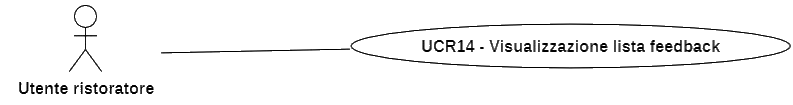
\includegraphics[width=0.8\textwidth]{./uml/UCR14.png} 
	\caption{Visualizzazione lista \textit{feedback}}
	\label{fig:UCR14}
  \end{figure}

\begin{itemize}
	\item \textbf{Attore principale:} Utente ristoratore.

	\item \textbf{Precondizione:} L'Utente ristoratore ha effettuato l'accesso al sistema (vedi \autoref{usecase:Effettua accesso}).

	\item \textbf{Postcondizione:} L'Utente ristoratore visualizza la lista di \textit{feedback} inseriti da vari clienti.


	\item \textbf{Scenario principale:}
	      \begin{enumerate}
		      \item L'Utente ristoratore accede alla sezione dedicata alla visualizzazione dei \textit{feedback};

		      \item Il Sistema mostra la lista di \textit{feedback};

		      \item Il Sistema mostra nome di chi ha scritto il \textit{feedback} e la data di pubblicazione;

		      \item L'Utente ristoratore visualizza tutti i \textit{feedback} e le informazioni legate ad esso.
	      \end{enumerate}
\end{itemize}
